
\section{X-Ray Diffraction}
    \label{Sec:3:XrayDiffraction}

The crystalline axes of the sample were determined on a Kappa Apex II single crystal diffractometer with the help of Mairi Haddow. The sample was mounted on a glass rod using vacuum grease during the measurements.
%%
\begin{figure}[h!]
    \begin{center}
        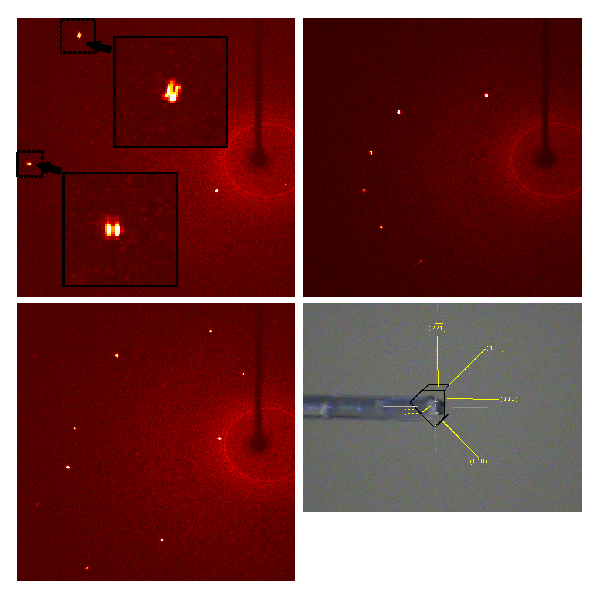
\includegraphics[scale=0.7]{Chapter3-dHvABaFe2P2/Figures/Xrays/XRayDiffraction/XrayDiffraction}
        \caption{Top left, top right and bottom left show example diffraction patterns of the \BaFeP sampple. Top-left shows a zoomed portion of doubled peaks indicating that there may potentially be a misalignment within the crystal. Bottom right shows the labeled crystal axes superimposed on the sample which is mounted on a glass rod.}
        \label{Fig:3:XRayDiffraction}
    \end{center}
\end{figure}

Table~\ref{Table:3:LatticeParams} shows the lattice parameters as determined by the x-ray measurements.
%%
\medskip
%% 
\begin{center}
    \begin{tabular}[h!]{llr}
\toprule
Source  &  $a$ (\AA) & $c$ (\AA) \\
\midrule
X-ray   & 3.82  & 12.38 \\
Mewis et al.\cite{Mewis1980} & 3.84 & 12.44 \\
Rotter et al.\cite{Rotter2010} & 3.84 & 12.42 \\
\bottomrule
    \label{Table:3:LatticeParams}
    \end{tabular}
\end{center}

